\documentclass[11pt,french]{report}

\usepackage[utf8]{inputenc}
\usepackage[french]{babel}
\usepackage{fontenc}
\usepackage{amsfonts}
\usepackage{amsmath}
\usepackage{graphicx}
\usepackage{bbm}
\usepackage[a4paper, margin=1.2in]{geometry}
\usepackage{hyperref}

\renewcommand{\thesection}{\Roman{section}}

\newcommand{\HRule}{\rule{\linewidth}{0.5mm}}
\addto\captionsfrench{\renewcommand{\chaptername}{Partie}}

\begin{document}
	\title{Rapport sur les algorithmes d'approximation et de méta-heuristique pour le problème de l'arbre de Steiner\\}
	\author{
		Éric Aubinais, Farid Najar\\[0.2cm]
		Master Mathématiques de l'Intelligence Artificielle }
	\date{Octobre 2020}
	\makeatletter
	\begin{titlepage}
		\centering
		\textsc{\LARGE Institut de Mathématiques d'Orsay \\ Université Paris-Saclay}\\[4cm]
		\HRule \\
		{ \huge \bfseries \@title[2cm] }
		\begin{Large}
			\@author
		\end{Large}
		\HRule
		\vfill
		
\includegraphics[width=0.35\textwidth]{paris-saclay.png}
		\hfill
		
\includegraphics[width=0.35\textwidth, height=2.5cm]{imo.png}
		\pagebreak
		\tableofcontents
		\pagebreak
	\end{titlepage}

	\section{Contexte\label{Contexte}}
	Imaginons que nous avons un réseau avec une source et plusieurs destinations. Nous voulons avoir des chemins depuis la source vers les destinations sans être coupé par d'autres chemins. Dit autrement, nous voulons un graphe sans cycle, i.e. un arbre, en partant de la source et en ayant les destinations qu'on veut visiter. De plus, pour aller d'un point à l'autre, il faut payer un coût. Le but est de trouver l'arbre qui vérifie les conditions énoncées de coût minimal.
	\section{Modélisation\label{Modélisation}}
	Nous pouvons modéliser le réseau par un graphe connexe $G = (V, E)$ avec $V$ l'ensemble des sommets et $E$ l'ensemble des arêtes. On introduit aussi une fonction $w:E\rightarrow \mathbb{N}$ qui à chaque arête $e\in E$ attribut un poids $w(e)$. Soit $T$ l'ensemble des "terminaux" qui sont tout simplement les destinations que nous avons énoncé. On remarque que la source peut être considérée comme un terminal. En effet, comme notre solution est un arbre, on peut le représenter comme on veut en prenant un nœud quelconque comme source. Alors notre problème est de trouver un arbre $A = (V', E')$ (graphe connexe sans cycle), tel que $T\subseteq V'$ et on veut minimiser \label{poids}{$\sum_{e\in E'}w(e)$}. On représente les solutions comme une liste de 0 ou 1 de taille $|E|$. En numérotant les arêtes, pour une solution $s$, $s_i$ nous dit si le $i$-ème arête est dans l'arbre ou pas (1 oui, 0 non).
	\section{Complexité\label{Complexité}}
        Selon la modélisation que l'on a décidé de prendre pour le problème de l'arbre de Steiner, celui-ci est NP-complet.

        \subsection{Steiner est NP}
        Étant donné une solution $A$ au problème énoncé ci-dessus, on peut vérifier en temps polynomial les éléments suivants :

        \begin{itemize}
	\item[1.] $A$ est bien un arbre connexe ne contenant aucun cycle
        \item[2.] $A$ couvre bien tous les sommets de $T$
	\end{itemize}

        Ce qui nous reste à vérifier est que cet arbre est minimal en terme de poids. On sait en particulier qu'il existe un algorithme de vérification pour ce problème qui se calcule en temps linéaire. Il en suit donc que ce problème est NP.

        \subsection{Steiner est NP-complet}
        Pour aboutir au fait que Steiner est NP-complet, on peut se baser sur une réduction du problème $Set Cover$ dans Steiner. En effet, ce dernier est connu pour être NP-complet.
        En partant d'une instance de $Set Cover$ pour $n$ points et $K$ ensembles, on peut construire une instance de Steiner. En effet, on procède comme suit :
        
        \begin{itemize}
	\item[1.] On considère trois étages de sommets :
          \begin{itemize}
          \item[a.] Le premier étage est consistitué d'un seul sommet, considéré comme terminal
          \item[b.] Le deuxième étage est consititué de $K$ sommets non terminaux
          \item[c.] Le troisième étage est constitué de $n$ sommets tous terminaux
          \end{itemize}
        \item[2.] le sommet du premier étage est relié à tous les sommets du second étage. Un sommet du second étage est relié à un sommet du dernier étage si et seulement si l'ensemble que représente le sommet du second étage contient le point que représente le sommet du dernier étage.
          \item[3.] Chacune des arêtes possède un poids dépendamment du problème
	\end{itemize}

        Si le problème de $Set Cover$ possède une solution pour $K$ alors il existe une solution pour Steiner avec $K' = n+K$

        En partant d'une solution de Steiner pour $K'$ du type le graphe présenté ci-avant, alors la solution pour $Set Cover$ avec $K$ est donnée.
        Supposons que l'on change une seule arête dans le graphe de Steiner. Le nouvel arbre que l'on obtient est toujours (de façon évidente car on change une seule arête) équivalent à un arbre du type présenté ci-avant. En procédant par récurrence, il en suit qu'on a toujours une solution de $Set Cover$ si on a une solution pour Steiner


        Ainsi, on a réussi à créer une réduction de $Set Cover$ dans Steiner avec $Set Cover$ NP-complet donc Steiner l'est
        
	\section{Algorithme d'approximation et taux d'approximation\label{Approx}}
	Comme le problème est NP-Complet, alors si on considère $P\neq NP$, on ne peut construire un algorithme donnant une solution optimale en temps polynomial. Dans ce cas, nous avons plusieurs façon de trouver une solution qui est proche ou, dans certain cas, égale à une solution optimale. Dans ce rapport, nous allons faire et évaluer deux de ces méthodes, "\textbf{approximation}" et "\textbf{méta-heuristique}". Commençons par l'approximation. Une approximation consiste à essayer, à l'aide de différentes techniques, de trouver la meilleure solution possible en temps polynomial avec une distance maximale déterminée par rapport à la solution optimale qui est appelé le \textbf{taux d'approximation} qui est un critère essentiel qui nous permet d'évaluer ce genre d'algorithmes. On peut construire un algorithme d'approximation de différentes manières. Dans cette section, nous allons voir une de ces manières.
	
	\subsection{Algorithme d'approximation\label{Algo approx}}
	Nous cherchons un arbre qui passe par tous les sommets terminaux. On remarque que trouver un tel arbre dans un graphe quelconque est équivalent à trouver cet arbre dans un graphe complet avec les terminaux comme sommet. En effet, si on construit ce graphe en mettant la distance minimale entre chaque sommet comme poids de l'arrête qui les relie, et trouver un arbre couvrant de poids minimum qui passe par tous les sommets, on est sûr que nous avons un arbre pour le graphe d'origine en passant par les terminaux. On doit aussi enregistrer les plus courts chemins dans la mémoire afin de ne pas être obligé de les recalculer, et ainsi, ajouter une complexité supplémentaire à notre algorithme. Pour récapituler, nous avons le procédé suivant : 
	\begin{itemize}
		\item[\textbf{1.}] On construit $G_+$ le graphe complet qui a les terminaux comme sommets et sur chaque arrête, on met le poids du plus court chemin. On enregistre, à chaque fois, le plus court chemin dans la mémoire. Pour calculer les plus courts chemins, on utilise l'algorithme Dijkstra.\\
		Complexité : On pose $n=|V|$. Pour Dijkstra, on a une complexité $O(n^2\log(n))$. Et pour le stockage des chemins, on a $O(n)$
		\\
		\item[\textbf{2.}] On construit $A$, l'arbre couvrant de poids minimum de $G+$. Cet algorithme a une complexité de $O(|T|\log(|T|))$.
		\\
		\item[\textbf{3.}] On renvoie l'union des arrêtes qui composent les plus courts chemins. Comme on a enregistré ces chemins, on une complexité $O(1)$.
	\end{itemize}
	
	\subsection{Taux d'approximation\label{taux}} 
	Soit $T^*$ une solution optimale. On sait déjà qu'une solution $C$ donnée par le cycle eulérien vérifie $C=2T^*$. On a solution $C'$ en prenant les sommets par ordre de première apparition et on a $C'\leq C$. Soit $A$ une solution de l'approximation. On a $A\leq C'$, car, on peut supprimer, au minimum, une arrête de $C'$ afin de ne pas avoir de cycles. Alors, on a $A\leq 2T^*$ par transitivité. Comme on renvoie l'union des arrêtes, on a $Resultat\leq A$. On a donc 2-approximation.
	
	\section{Méta-heuristiques\label{Méta-heuristiques}}
	L'approximation est une bonne façon de trouver les solutions, mais, il n'est pas évident de trouver un algorithme d'approximation. Dans cette section, nous allons voir deux algorithmes, de la famille des algorithmes méta-heuristiques, qui sont probabilistes et donnent des résultats différents à chaque exécution. L'intérêt de ces algorithmes est dans leur flexibilité et la facilité d'implémentation. En effet, contrairement au cas d'approximation, nous n'avons pas besoin de chercher une manière spécifique de trouver la meilleure solution. Dans de nombreux cas, on n'a toujours pas trouver un algorithme d'approximation et dans tant d'autres, les taux d'approximations sont assez élevés. Pour utiliser mes méta-heuristiques, il suffit d'adapter les algorithmes au problème et utiliser le plus pertinent selon les cas.\\
	
	Les méta-heuristiques partent d'une solution aléatoire et cherchent de nouvelles solutions en transformant la solution de base. Ensuite, elles évaluent ces solutions et gardent la ou les meilleures. Elles répètent cette opération un nombre de fois qu'il faut déterminer. Finalement, elles rendent la meilleure qu'ils ont trouvé.\\
	
	Pour notre problème, nous avons choisi deux algorithmes que nous avons jugé pertinents pour ce dernier. Deux algorithmes qui viennent de deux familles différentes de ce genre. Le premier fait partie de la famille \textbf{méta-heuristiques à parcours} et \textbf{méta-heuristiques à population}. Ces deux algorithmes, comme la plupart des algorithmes de ce genre, se sont inspirés des phénomènes naturels.
	
	\subsection{Algorithme recuit\label{recuit}}
	L'algorithme recuit, qui fait parti des méta-heuristiques à parcours, s'inspire du recuit des métaux afin de modifier les caractéristiques de ces derniers. Le procédé consiste à chauffer le métal à une température précise et ensuite le refroidir d'une manière contrôlé. Cela nous aide à contourner certaines contraintes physiques.\\
	
	Dans notre cas, ce procédé peut nous aider à ne pas rester coincé dans un minimum/maximum local. En effet, nous parcourrons l'espace des solutions afin de trouver le plus petit coût. À cause de ça, si on fait un parcours normal comme "hill climbing", on peut se trouver proche d'un minimum local qui n'est pas global et ainsi, ne pas avoir des performances souhaitées. Cependant, il faut faire attention aux températures très élevées, car, elles peuvent nous éloigner de la solution optimale.\\
	
	Nous devons aussi savoir contrôler le refroidissement. Un refroidissement très rapide peut causer des résultats loin de la solution optimale, et un refroidissement très lent peut prolonger le comportement chaotiques des températures élevées et causer un temps de calcule très élevé.
	
	\subsubsection{Recuit simple\label{recuit simple}}
	Dans le recuit simple, on a un seul "chercheur" pour la solution. 
	L'algorithme initial pour un refroidissement exponentiel de paramètre $\lambda$ et une température initiale $T_{init}$ et une température limite $T_{limit}$ est :\\
	
	\begin{itemize}
        \item[1.] On part d'une solution aléatoire et on la nomme $best$. On pose $T = T_{init}$
		\item[2.] On génère un voisin aléatoire nommé $voisin$.
		\item[3.] On évalue les deux
		\item[4.] Si le voisin a une meilleure évaluation, ici meilleure c'est plus petit, on pose $prob = 1$ et on va à la ligne 6.
		\item[5.] Sinon, on pose $prob = e^{-\frac{(evaluation(voisin) - evaluation(best))}{T}}$
		\item[6.] On tire un nombre aléatoire nommé $rand$ entre 0 et 1 suivant la loi uniforme.
		\item[7.] Si $rand < prob$ alors $best = voisin$
		\item[8.] T = $\lambda T$
		\item[9.] Si $T<T_{limit}$ on part à la ligne 2 sinon on arrête et on renvoie $best$\\
	\end{itemize}

	Notez que dans le terme de l'exponentielle, on a aussi la constante de Boltzmann au dénominateur qui est égal à 0 dans notre algorithme. 
	Remarquons que la température a une influence direct sur $prob$ et si on a une température élevé, $prob$ va être proche de 1, donc, on a une forte probabilité de changer $best$ même si l'évaluation de $voisin$ n'est pas meilleure. Cela explique les fluctuations à températures élevée et la nécessité de décroître la température rapidement vers un niveau stable. C'est pour cette raison que nous avons choisi une décroissance exponentielle de la température qui nous assure ce dernier critère, et en même temps, laisse un peu de temps à l'algorithme pour converger vers le minimum le plus proche.\\
	
	Pour générer un voisin aléatoire, nous prenons une indice aléatoirement et on change $i$-ème valeur, de sorte que, si c'est 0, on met 1, sinon, on met 0.\\
	
	Pour évaluer les solutions, on prend déjà \hyperref[poids]{la somme des poids} dans la section modélisation, de plus comme on ne veut pas de solutions invalides, on les pénalise avec un coefficient grand nommé $malus$. Dans notre algorithme, nous avons pris $malus = 500$ afin de mettre une différence remarquable entre les solutions valides et invalides. Les solutions invalides sont les solutions qui ne sont pas des arbre ou elles ne contiennent pas les terminaux ou ne sont pas connexes. Autrement dit, on doit compter le nombre de composants connexes dans le graphe engendré par la solution et le nombre de terminaux absent dans ce même graphe. On peut s'en passer des cycles, car, ils sont déjà pénalisés dans la somme des poids. Pour le nombre de terminaux absents, on a doublé le malus, car, avoir des terminaux absents dans la solution est très grave. On a donc avec $absents$ qui représente les terminaux absents et $connexes$ qui représente les nombre de composantes connexes : 
	$$
	evaluation = 1000*absents + 500*(connexes-1)+ \sum_{e\in E'}w(e)
	$$\\
	
	
	Pour l'algorithme initial, nous avons pris $\lambda = 0.99$. Cependant, afin de permettre une convergence vers le minimum, dans la version finale nous changeons $\lambda$ à partir d'une température $T_{seuil}$. Grâce à ce changement, on a un meilleur résultat, mais, on rallonge le temps de calcul. Voici la version finale :\\
	\begin{itemize}
		\item[1.] On part d'une solution aléatoire et on la nomme $best$. On pose $T = T_{init}$
		\item[2.] On génère un voisin aléatoire nommé $voisin$.
		\item[3.] On évalue les deux
		\item[4.] Si le voisin a une meilleure évaluation, ici meilleure c'est plus petit, on pose $prob = 1$ et on va à la ligne 6.
		\item[5.] Sinon, on pose $prob = e^{-\frac{(evaluation(voisin) - evaluation(best))}{T}}$
		\item[6.] On tire un nombre aléatoire nommé $rand$ entre 0 et 1 suivant la loi uniforme.
		\item[7.] Si $rand < prob$ alors $best = voisin$
		\item[8.] T = $\lambda T$
		\item[9.] Si $T<T_{seuil}$ alors $\lambda = \lambda_{alternative}$
		\item[10.] Si $T<T_{limit}$ on part à la ligne 2 sinon on arrête et on renvoie $best$
	\end{itemize}
	
	\subsubsection{Recuit multiple\label{recuit multiple}}
	Seul on va plus vite, ensemble, on va plus loin ! Cette expression résume bien l'intérêt d'avoir plusieurs chercheurs. Avec un temps de calcul un peu plus long, on peut avoir des résultats plus intéressants que recuit simple. Pour cela, au lieu de partir d'une solution aléatoire, on part de $n$ solutions aléatoires qu'on met dans une liste nommée $bests$. On utilise la même évaluation que recuit simple.\\
	
	\begin{itemize}
		\item[1.] On part de $n$ solutions aléatoires et on la nomme $bests$. On pose $T = T_{init}$
		\item[2.] On fait les étapes 2 à 9 de recuit simple pour chaque membre de $bests$
		\item[3.] Si $T<T_{limit}$ on part à la ligne 2 sinon on arrête et on renvoie la solution qui a la meilleure évaluation parmi les membres de $bests$.\\
	\end{itemize}
	
	Nous allons voir dans la section résultats la différences entre ces deux versions.
	
	\subsection{Algorithme génétique\label{Génétique}}
	Faisant partie de la famille des méta-heuristiques à populations, il s'inspire aussi d'un phénomène naturel, l'évolution et la sélection naturelle. On part encore d'une solution aléatoire et on crée une population de solutions avec une méthode "\hyperref[Génération]{génération}". Puis, à l'aide de l'évaluation vu dans \hyperref[recuit simple]{recuit}, on \hyperref[sélection]{sélectionne} les meilleures. On répète ce procédé un nombre défini de fois. On garde la même représentation de solution.
	
	\subsubsection{Génération\label{Génération}}
	Pour générer de nouvelles solutions, on s'inspire de la reproduction naturelle. D'abord on croise deux solutions, ensuite, on prend une indice aléatoire et on mute la valeur à cette indice, $i.e.$, on met 0 si c'est 1, sinon, 1. Cependant, comme nos simulations nous l'ont montrer, cette méthode peut s'avérer lente en convergence vers la solution optimale, car, elle ne génère pas assez de solutions. Il faut donc accélérer le processus. Alors, au lieu de muter seulement les nouveaux nés, on génère aussi une copie mutée de toutes les solutions de la populations. Ainsi, on évaluent beaucoup plus de solutions à chaque fois et on a une meilleure chance pour trouver la meilleure solution.\\
	
	Pour le croisement, on croise systématiquement les deux meilleures solutions. Encore une fois, on s'est inspiré de la nature, parce que dans beaucoup d'espèces, seul le couple alpha ont le droit de se reproduire. On génère un premier enfant qui a la première moitié du parent 1 et la deuxième moitié du parent 2. Pour le deuxième enfant, on fait l'inverse, $i.e.$, la première moitié vient du parent 2 et la deuxième du parent 1. Mais nous ne nous sommes pas contenté du couple alpha et à chaque reproduction, nous prenons aléatoirement deux solutions et on les croise. Grâce à cela, on peut avoir une population plus variée.
	
	\subsubsection{Sélection\label{sélection}}
	Pour la sélection, on doit d'abord choisir le nombre maximum de solutions qu'on veut garder nommée $m$. On doit pas prendre $m$ très petit, sinon, on risque de ne pas générer des solutions variées, et ainsi, ne pas converger vers la solution optimale. On ne doit pas prendre $m$ très grand, sinon, on risque d'augmenter drastiquement le temps de calcul. Nous avons choisi $m=15$ pour avoir une population assez grande afin évaluer un grand nombre de solutions, et assez petit pour être raisonnable en temps de calcul. Ce nombre a été trouver par tâtonnement à l'aide des simulations.
	
	\subsubsection{Algorithme}
	Soit $n$ le nombre d'itération.
	
	\begin{itemize}
		\item[1.] On part d'une solution aléatoire et on la nomme $best$.
		\item[2.] On génère une nouvelle \hyperref[Génération]{génération}
		\item[3.] On \hyperref[sélection]{garde} les $m$ meilleures.
		\item[4.] Si le meilleur de la population est meilleur que $best$, alors, on remplace $best$.
		\item[5.] On répète $n$ fois à partir de 2.
		\item[6.] On renvoie $best$
	\end{itemize}
	
	
	\section{Résultats et performances}

        Dans l'optique d'obtenir les résultats expérimentaux les plus performants possible, il est nécessaire de faire varier les différents paramètres des algorithmes de plusieurs façons différentes, afin des les ajuster le plus précisément possible. Pour étudier l'efficacité d'un algorithme, dépendamment de ce que l'on veut, on peut vouloir avoir des performances de précision, des performances de rapidité d'exécution ou encore des performances de convergence (dans le sens où l'algorithme peut prendre du temps à s'exécuter mais utilise que peu d'itérations).


        \subsection{Algorithme recuit}

        Pour cet algorithme, il est possible de faire varier ses performances en faisant varier la température initiale $T_{init}$, faire varier le paramètre $\lambda$ (en argument ou dans le code même) ou encore utiliser la version multiple de cet algorithme.

        \subsubsection{Température initiale}
        
        \begin{figure}
        	\begin{center}
        		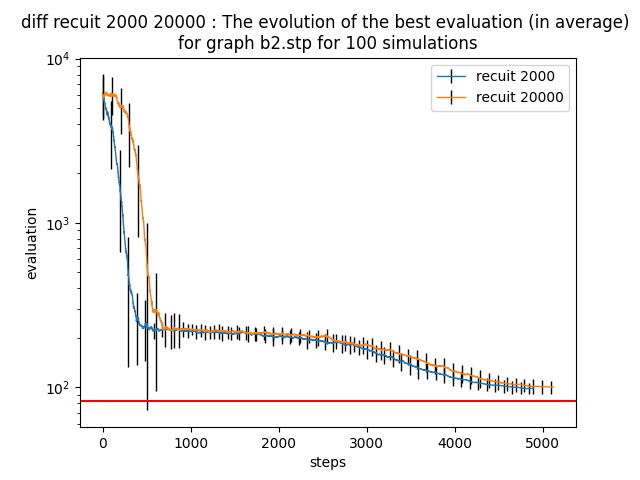
\includegraphics[width=0.8\textwidth]{best_b2_evaluation_diff recuit 2000 20000.png}
        	\end{center}
        	\caption{Simulation sur b2 de l'algorithme recuit avec deux températures différentes}
        	\label{Figure1}
        \end{figure}
        
        \hyperref[Figure1]{(Figure 1)} montre en particulier la différence de convergence entre un algorithme de recuit avec température initiale 2000 ou 20000. Ce graphique nous montre en particulier que la température initiale va modifier la vitesse de convergence de l'algorithme. Plus la température est élevée, plus le début sera lent. Par ailleurs, plus la température initiale est élevée, plus le temps d'exécution de l'algorithme sera long pour un résultat relativement identique.
        Par conséquent, il est préférable, dans une circonstance de rapidité d'exécution de l'algorithme, d'initialiser la température à 2000.
        En revanche, bien que la convergence ait toujours lieu avec des températures initiales inférieures, fixer la température à 2000 est un juste milieu entre le temps d'exécution de l'algorithme et la stabilité des solution. En effet, une température inférieure donnera plus de chance à une divergence de la solution.\\
        
        %\begin{figure}
        %\begin{center}
        %	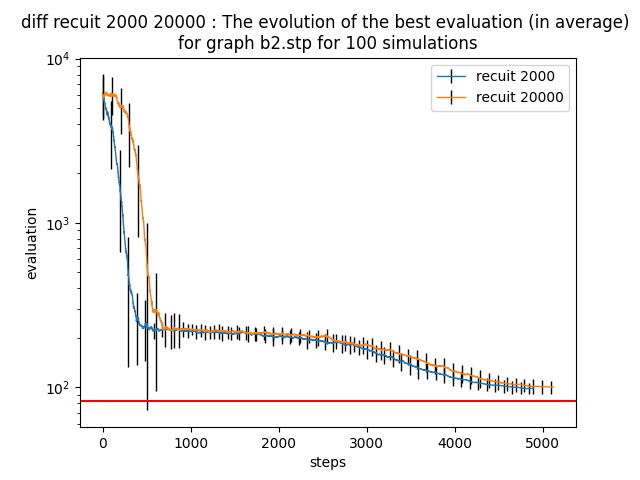
\includegraphics[width=1\textwidth]{best_b2_evaluation_diff recuit 2000 20000.png}
        %\end{center}
%        	\caption{Simulation sur b2 de l'algorithme recuit avec deux températures différentes}
        %\end{figure}

        \subsubsection{Paramètre lambda}
        La température initiale fixée à 2000, on compare dans la \hyperref[Figure2]{figure 2} la convergence du recuit pour $\lambda$ fixé à 0.99 ou 0.999 sans variation interne et la convergence du recuit pour $\lambda$ fixé à 0.99 l'un sans variation interne et l'autre avec.
        \begin{figure}
        		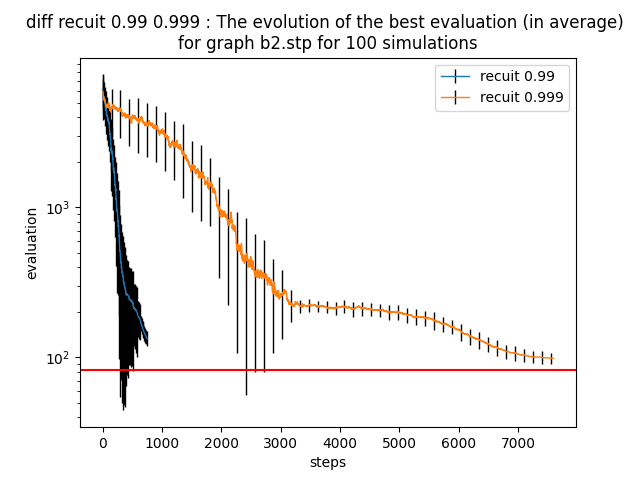
\includegraphics[width=0.5\textwidth]{best_b2_evaluation_diff recuit 0.99 0.999.png}
        		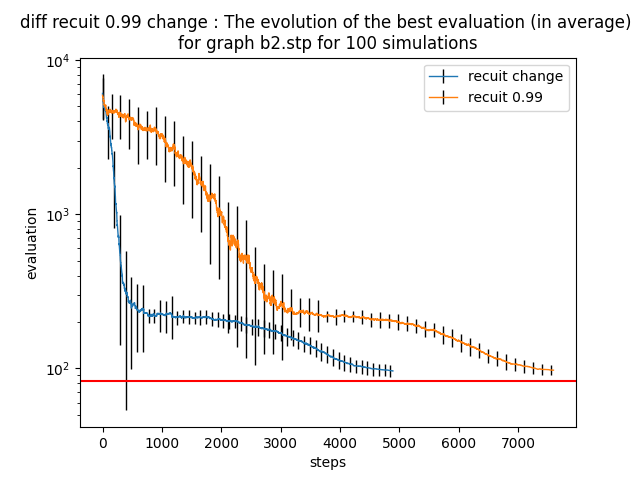
\includegraphics[width=0.5\textwidth]{best_b2_evaluation_diff recuit 0.99 change.png}
        	\caption{Simulation sur b2 de l'algorithme recuit avec deux lambda différents}
        	\label{Figure2}
        \end{figure}
        
%        \begin{figure}
 %       	\begin{center}
  %      		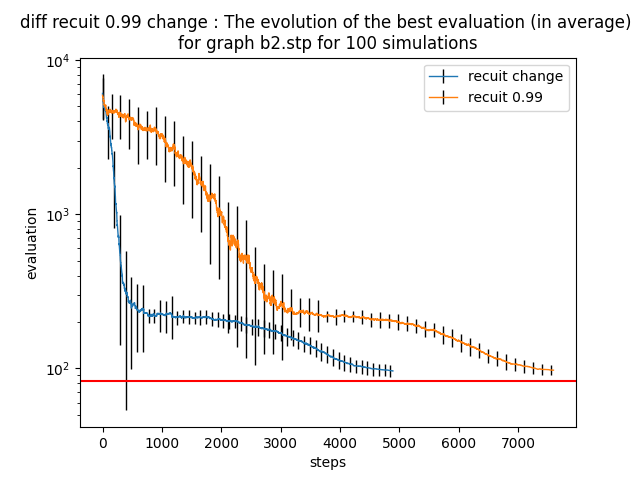
\includegraphics[width=0.5\textwidth]{best_b2_evaluation_diff recuit 0.99 change.png}
   %     	\end{center}
    %    	\caption{Simulation sur b2 de l'algorithme recuit avec deux lambda différents}
     %   	\label{Figure3}
      %  \end{figure}
        Le premier graphe (\hyperref[Figure2]{(Figure 2)}) nous montre en particulier que l'algorithme prendra plus de temps à converger avec un lambda fixé à 0.999 mais convergera vers une solution plus précise. Le second graphe nous montre que l'alternative de changer en cours de route la valeur de $\lambda$ est un compromis très efficace entre rapidité et précision. En effet, la valeur obtenu est meilleure avec le changement que sans, et l'algorithme converge plus rapidement. 

        Par conséquent il est préférable d'utiliser la version faisant varier le $\lambda$ dans l'algorithme.

        \subsubsection{Version multiple}
        On fixe à présent la température initiale à 2000, le paramètre $\lambda$ à 0.99 (en considérant le changement du $\lambda$ dans l'algorithme).
        Le graphe suivant \hyperref[Figure3]{(figure 3)} compare l'algorithme de recuit à celui de recuit multiple pour un nombre de chercheur fixé à 5.
        \begin{figure}
          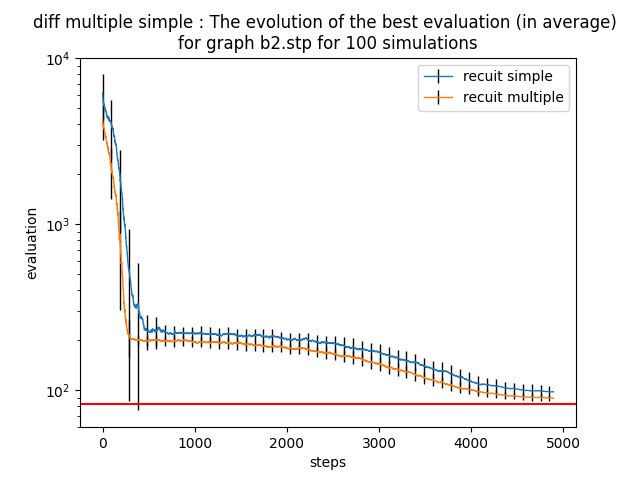
\includegraphics[width=0.5\textwidth]{best_b2_evaluation_diff multiple simple.png}
          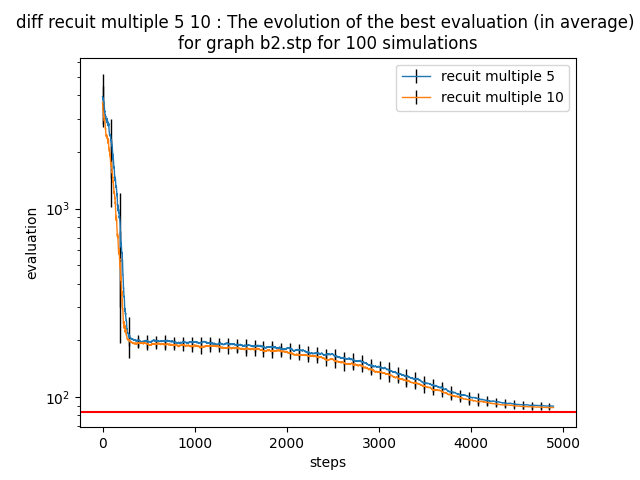
\includegraphics[width=0.5\textwidth]{best_b2_evaluation_diff recuit multiple 5 10.png}
          \caption{Simulation sur b2 de l'algorithme recuit simple et recuit multiple}
          \label{Figure3}
        \end{figure}

        Ce graphique nous montre que sur le point de vitesse de convergence et de précision de convergence, l'algorithme de recuit multiple est bien plus performant que le recuit simple. Il est par conséquent préférable, si on cherche ces performances, de choisir l'algorithme multiple. En revanche, en dénotant $n$ le nombre de chercheur pour l'algorithme multiple, ce dernier prend environ pour une simulation $n$ fois plus de temps que le recuit simple.L'algorithme de recuit simple réalisant résultat tout de même très satisfaisant, il peut être préférable de choisir le recuit simple si la rapidité d'exécution est la priorité.

        Il est notable aussi de noter que $n$=5 est une valeur efficace pour l'algorithme de recuit multiple. En effet, comme le montre le graphe de droite de \hyperref[Figure3]{(Figure 3)}, il n'y a pratiquement pas de différence entre $n=5$ et $n=10$, si ce n'est le temps d'exécution (bien inférieure pour $n$=5)


        De ce qui précède, il est donc totalement préférable si l'on cherche une performance de convergence, de choisir l'algorithme de recuit multiple avec pour paramètres $T_{init} = 2000$,  $\lambda = 0.99$ et $n=5$, tandis que si l'on cherche une performance de rapidité d'exécution, il est préférable de choisir l'algorithme de recuit simple avec pour paramètres $T_{init} = 2000$ et $\lambda = 0.99$ avec changement à l'intérieur du code.


        \subsection{Algorithme génétique}
        Pour cet algorithme, il est possible de faire varier ses performances en faisant varier l'initialisation (fonction $init$) ou le paramètre $maxpop$.

        \subsubsection{Initialisation}
        
        Une multitudes d'initialisation sont possibles pour cet algorithme. On pourrait, bien que nous ne le faisons pas dans cette section, initialiser notre algorithme avec une approximation déjà faite. Le but étant que notre algorithme soit appliqué sur notre jeu de donnée sans étude préalable, on a opté pour une initialisation sans approximation préalable. Les graphes de la \hyperref[Figure4]{(Figure 4)} montrent en particulier que l'initialisation aléatoire est la meilleure.

        \begin{figure}
          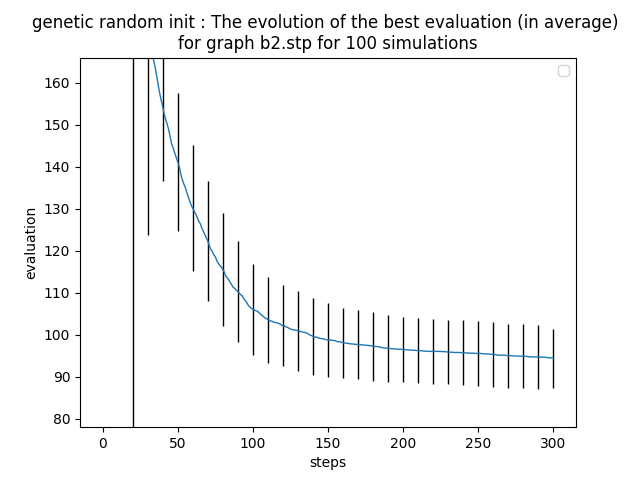
\includegraphics[width=0.33\textwidth]{best_b2_evaluation_genetic random init.png}
          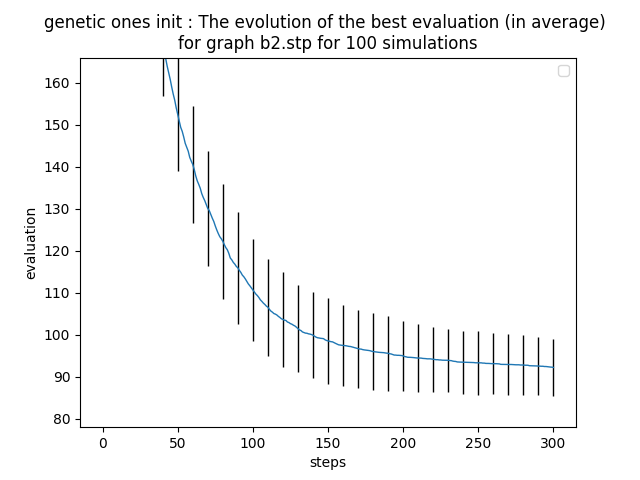
\includegraphics[width=0.33\textwidth]{best_b2_evaluation_genetic ones init.png}
          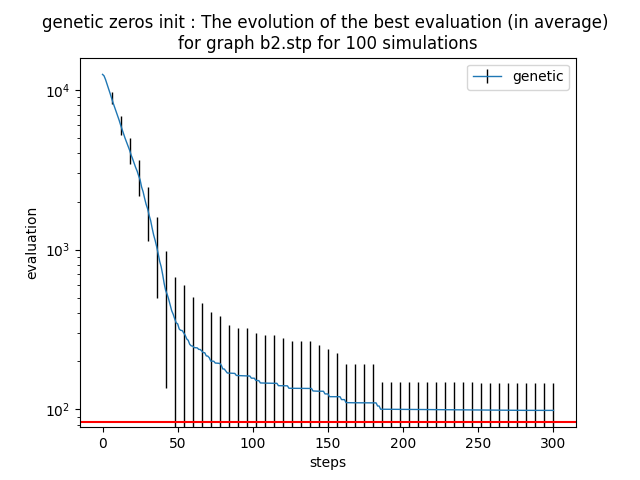
\includegraphics[width=0.32\textwidth]{best_b2_evaluation_genetic zeros init.png}
          \caption{Simulation sur b2 de l'algorithme génétique avec différentes initialisations}
          \label{Figure4}
        \end{figure}
        

        En effet, il est clair que l'initialisation uniquement avec des zéros ne convient absolument pas dû aux barres d'erreurs très grandes qu'il présente. Cela veut dire en particulier qu'il y a beaucoup de cas qui ne converge pas bien. De plus, on voit ici que l'algorithme initialisé aléatoirement converge plus rapidement avec des barres d'erreur bien plus petites que celui initialisé qu'avec des 1.
        Il est ainsi préférable d'utiliser une initialisation aléatoire.

        \subsubsection{Max population}
        On considère donc une initialisation aléatoire. Le graphe de gauche de  \hyperref[Figure5]{(Figure 5)} nous permet de comprendre qu'à partir d'un certain palier, changer la valeur de $maxpop$ n'apporte rien à l'algorithme, tout en le ralentissant fortement.

        \begin{figure}
          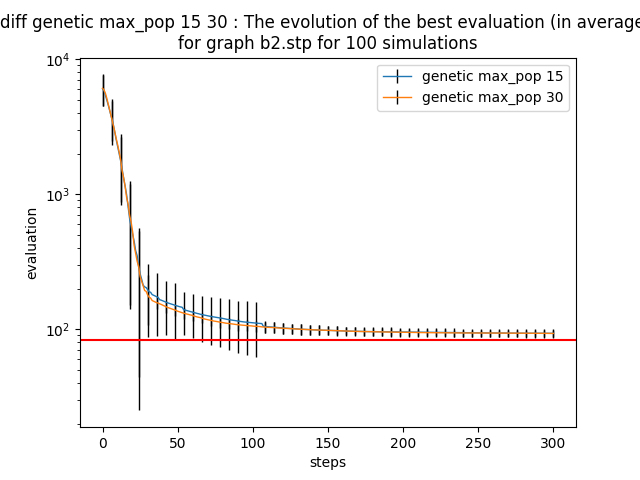
\includegraphics[width=0.5\textwidth]{best_b2_evaluation_diff genetic max_pop 15 30.png}
          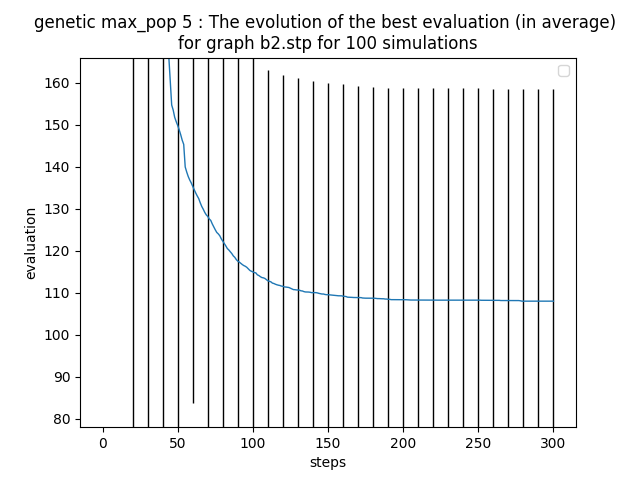
\includegraphics[width=0.5\textwidth]{best_b2_evaluation_genetic max_pop 5.png}
          \caption{Simulation sur b2 de l'algorithme génétique avec différentes valeurs de max population}
          \label{Figure5}
        \end{figure}

        En revanche, le graphe de droite de \hyperref[Figure5]{(Figure 5)} nous montre qu'avec une population maximale trop faible, les barres d'erreurs deviennent relativement grandes. Cela signifie que l'algorithme est moins efficace en général.

        Ainsi, une population maximale de 15 semble être la valeur optimale pour cet algorithme.


        De ce qui précède, peu importe les circonstances, les paramètres optimaux pour l'algorithme génétique sont $init = random$ et $maxpop = 15$.

        \subsection{Comparaison}
        Étant donné que l'on a identifié pour les deux algorithmes les paramètres optimaux, il peut être intéressant de connaître lequel est le plus performant.

        \begin{figure}
          \begin{center}
            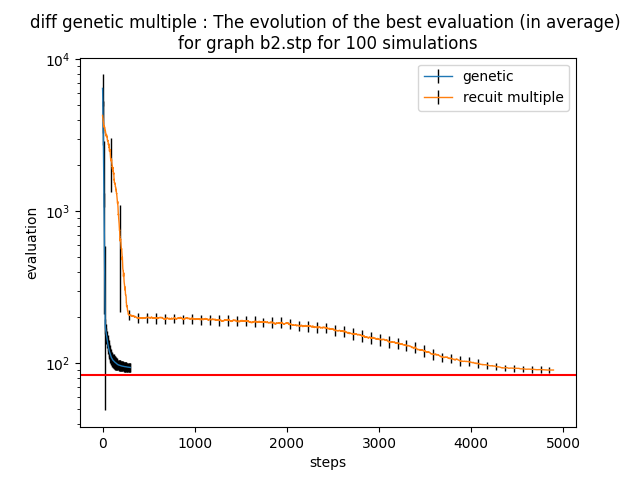
\includegraphics[width=0.8\textwidth]{best_b2_evaluation_diff genetic multiple.png}
          \end{center}
          \caption{Simulation sur b2 de l'algorithme recuit simple et recuit multiple}
          \label{Figure6}
        \end{figure}

        Le graphe de la \hyperref[Figure6]{(Figure 6)} nous montre que les deux vont converger vers à peu près la même valeur, en ayant à peu près les mêmes barres d'erreurs. En revanche, en terme de vitesse de convergence, l'algorithme génétique est plus performant que recuit.
        Une analyse sur différents jeux de données nous a permis de voir que pour des taille relativement petite de jeux de données, l'algorithme génétique sera plus rapide que le recuit. Par exemple, sur une simulation sur le jeu de donnée b2.stp, génétique a pris moins d'une seconde pour s'exécuter tandis que recuit en a pris près de 4.
        En revanche, plus le jeu de donnée sera conséquent, moins l'algorithme génétique sera rapide. En effet, sur le jeu de donnée c1.stp contenant 500 nœuds, génétique a pris à peu près 45 secondes tandis que recuit s'est exécuté pendant un peu moins de 35 secondes.


        \subsection{Conclusion}

        \begin{figure}
          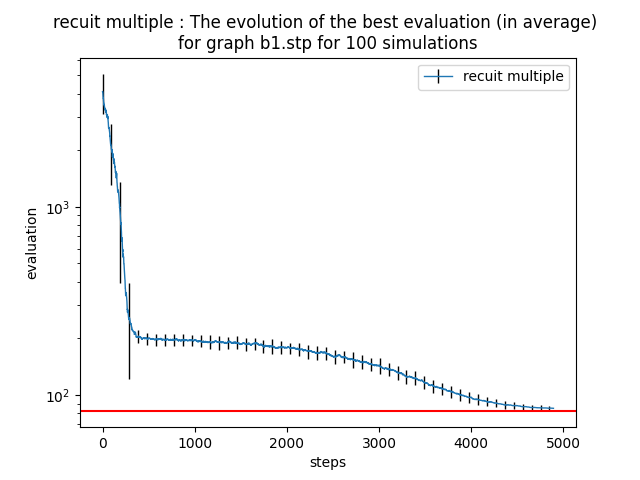
\includegraphics[width=0.5\textwidth]{best_b1_evaluation_recuit multiple.png}
          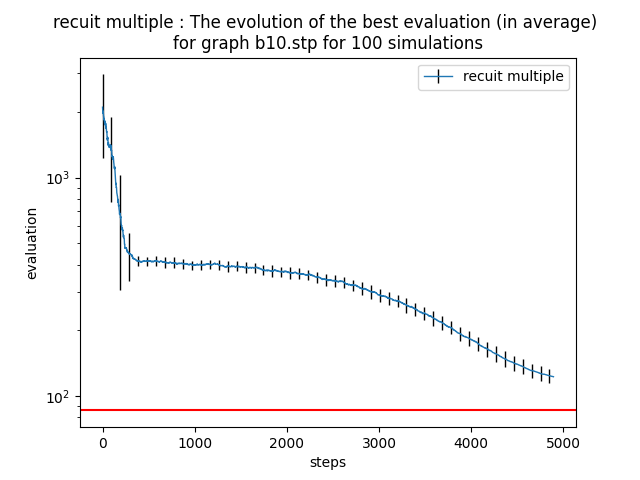
\includegraphics[width=0.5\textwidth]{best_b10_evaluation_recuit multiple.png}
          \caption{Simulation de l'algorithme recuit sur b1 et b10}
          \label{Figure7}
        \end{figure}

        On peut ainsi conclure, en observant sur la \hyperref[Figure7]{(Figure 7)} que l'algorithme de recuit multiple est probablement le mieux, étant donné que l'on a généralement des très gros jeux de données, et qu''il converge de façon assez précise même sur d'autres graphes.
        
%%%%%%%%%%%%%%%%%%%%%%%%%%%%%%%%%%%%%%%%%%%%%%%%%%%%%%%%%%%%%%%%%%%%%%%%%%%%%%%%%%%%%%%%%%%%%%%%%%
\end{document}
